%\documentclass[extra]{gji}
\documentclass[extra, referee]{gji}

\usepackage[utf8]{inputenc}
\usepackage{timet}
\usepackage{amsmath}
\usepackage{graphicx}

\usepackage{url}
\usepackage[pdftex,colorlinks=true]{hyperref}
\hypersetup{
    allcolors=blue,
}


\begin{document}

\title[Variable Density Tesseroids]{
    Gravitational field calculation in spherical coordinates using variable
    densities in depth
}
\author[S.R. Soler, A. Pesce, L. Uieda and M.E. Gimenez]{
    Santiago R. Soler$^{1,2}$, Agustina Pesce$^{1,2}$, Leonardo Uieda$^3$ and
    Mario E. Gimenez$^{1,2}$ \\
    $^1$CONICET, Argentina.~e-mail: santiago.r.soler@gmail.com\\
    $^2$Instituto Geofísico Sismológico Volponi, Universidad Nacional de
    San Juan, Argentina\\
    $^3$Department of Earth Sciences, SOEST, University of Hawai‘i at
    M\={a}noa, Honolulu, Hawaii, USA
}


\maketitle

\begin{summary}
We present a new methodology to compute the gravitational fields generated by
tesseroids (spherical prisms) whose density varies with depth according to
an arbitrary continuous function.
It approximates the gravitational fields through the Gauss-Legendre Quadrature along
with two discretization algorithms that automatically control its accuracy by adaptively
dividing the tesseroid into smaller ones.
The first one is a preexisting two dimensional adaptive discretization algorithm that
reduces the errors due to the distance between the tesseroid and the computation point.
The second is a new density-based discretization algorithm that
decreases the errors introduced by the variation of the density function with depth.
The amount of divisions made by each algorithm is indirectly controlled
by two parameters: the distance-size ratio and the delta ratio.
We have obtained analytical solutions for a spherical shell with radially variable
density and compared them to the results of the numerical model for linear and
exponential density functions.
These comparisons allowed us to obtain optimum values for the distance-size and
delta ratios that yield an accuracy of 0.1\% of the analytical solutions.
The resulting optimal values of distance-size ratio for the gravitational potential, its
gradient, and Marussi tensor are 1, 2 and 8, respectively.
A delta ratio of 0.2 is needed for the computation of the gravitational potential and
its gradient components, while a value of 0.01 must be used for the Marussi tensor
components.
Lastly, we apply this new methodology to model the Neuqu\'en Basin, a foreland basin in
Argentina with a maximum depth of over 5000 m, using an exponential density function.
\end{summary}

\begin{keywords}
Numerical modelling, Numerical approximations and analysis, Gravity anomalies
and Earth structure, Satellite gravity
\end{keywords}


\section{Introduction}

The lithosphere's density variation with depth has been studied for close to a
century.
Over this time period,
several density-depth relations have been proposed for different rock types
\citep[e.g.][]{Maxant1980, Rao1986, Rao1993, Rao1994}.
Furthermore, depth-variable densities have been used in forward and
inverse gravity modelling, mostly applied to sedimentary basins
\citep{Cordell1973, Rao1986, Cowie1990, Rao1993, Rao1994, Zhang2001,
Welford2010}.
These forward gravity models have been developed for two or three dimensional
bodies in Cartesian coordinates, which limits the applications to local scales.
The advent of satellite gravimetry has provided gravity field
measurements with global coverage, enabling modelling and interpretation on regional and
global scales.
Hence, designing forward modelling methods that reproduce the gravity anomalies for
such scales is of high importance.

To take into account the curvature of the Earth, many global forward modelling methods
are defined in geocentric spherical coordinates.
A common approach is to discretize the Earth into tesseroids (spherical prisms),
which are defined by pairs of latitude, longitude, and
radial boundaries (see Fig.~\ref{fig:tesseroid}).
The gravitational fields generated by an arbitrary
tesseroid on any external point are given by volume
integrals that must be numerically approximated.
The literature offers two main approaches: one involves Taylor series expansion
\citep{Heck2007, Grombein2013} while the other makes use of Gauss-Legendre
Quadrature (GLQ)
\citep{Asgharzadeh2007, Wild-Pfeiffer2008, Li2011, Uieda2016}.
The Taylor series expansion is not well suited to develop an algorithm for
a density varying with depth according to an arbitrary continuous function.
Different series expansion terms would have to obtained for each density function
desired.
Conversely, an arbitrary continuous density function can be included in the GLQ without
any change to the integration method.

\begin{figure}
\centering
\includegraphics[width=0.6\linewidth]{figures/tesseroid-uieda.pdf}
\caption{
    A tesseroid (spherical prism) in a geocentric spherical coordinate system, with a
    computation point $P$ and its local north oriented Cartesian coordinate system.
    After \citet{Uieda2015}.
}
\label{fig:tesseroid}
\end{figure}

The main challenge of the GLQ integration is loss of accuracy when the computation point
gets closer to the tesseroid \citep{Ku1977}.
\citet{Uieda2016} built on the three dimensional adaptive discretization algorithm of
\citet{Li2011} to automatically obtain integration results with 0.1\% accuracy.
The algorithm consist in recursively splitting the tesseroid into smaller ones when a
threshold is exceeded,
namely when the normalized distance to the computation point is greater than a
``distance-size ratio'' ($D$).
\citet{Uieda2016} have also obtained standard values of $D$
for the gravitational potential, its gradient and Marussi tensor components
by comparing the numerical model with the fields generated by a spherical shell.

Two recent papers present other approaches for homogeneous tesseroids gravitational
fields computation and incorporate methodologies for variable density tesseroid with
specific density profiles.
\citet{Fukushima2018} analytically integrates the volumetric integral for the
gravitational potential in the radial direction, obtaining a surface integral, which is
then numerically solved by applying a conditionally splitting and the double exponential
quadrature rule. The gradient of the potential and the Marussi tensor components are
then computed by finite differences. \citet{Fukushima2018} also generalizes his method
to an arbitrary polynomial density profile on the radial coordinate.
\citet{Lin2018} made a comparison of the different methodologies for homogeneous
tesseroid gravitational fields computation by applying different discretizations
algorithms to each one of them.
From this analysis they develop a combined method:
for computation points near the tesseroid they apply a GLQ numerical integration with
a two dimensional adaptive discretization algorithm, i.e.~only in the horizontal
dimension. But, if the computation point is farther than a certain truncation distance,
then a second order Taylor series approximation is applied along with the regular
subdivision developed by \citet{Grombein2013}.
They also introduce a variation of their combined method to compute the gravitational
fields generated by tesseroids with linear density on the radial coordinate.

In summary, the bibliography is offering different methodologies for computing
gravitational fields of homogeneous tesseroids or with certain specific density
functions in depth.
Although any continuous density profile could be approximated by one of these specific
density functions, one should acknowledge the error that such approximation would
propagate into the gravitational field in order to guarantee certain degree of accuracy.

We present a new algorithm for computing the gravitational fields generated by any
tesseroid with any arbitrary continuous density function on any external point.
It is based on the three dimensional GLQ approximation, a two dimensional version of the
adaptive discretization of \citet{Uieda2016} and a new density-based discretization
algorithm that we introduce in this work.
In order to ensure the accuracy of the numerical approximation we have
determined optimal values for the controlling parameters by
comparing the numerical approximation with analytical solutions for
spherical shells.
Finally, we applied the methodology to model the Neuqu\'en basin, Argentina, using
tesseroids with linear and exponentially increasing density with depth.


%%%%%%%%%%%%%%%%%%%%%%%%%%%%%%%%%%%%%%%%%%%%%%%%%%%%%%%%%%%%%%%%%%%%%%%%%%%%%%

\section{Methodology}

Consider an arbitrary tesseroid in a geocentric spherical coordinate system defined by
pairs of geocentric latitudinal ($\phi_1$, $\phi_2$), longitudinal ($\lambda_1$,
$\lambda_2$) and radial ($r_1$, $r_2$) boundaries.
We define an external computation point $P(r, \phi, \lambda)$ located at radius $r$,
geocentric latitude $\phi$, and longitude $\lambda$ where the gravitational fields the
tesseroid generates are going to be calculated.
The first- and second-order derivatives of the gravitational potential are taken with
respect to the local north-oriented Cartesian coordinate system of $P$
(Fig.~\ref{fig:tesseroid}).
\citet{Grombein2013} provide efficient formulations for the volume integrals of the
gravitational potential and its first- and second-order derivatives of a tesseroid with
homogeneous density.
Here, we will assume that the tesseroid has a density varying with $r$ according to an
arbitrary continuous function $\rho(r)$.
Thus, the integrals for the gravitational fields are slightly modified to

\begin{equation}
    V(r,\phi,\lambda) = G
    \int\limits_{\lambda_1}^{\lambda_2}
    \int\limits_{\phi_1}^{\phi_2}
    \int\limits_{r_1}^{r_2}
    \frac{\rho(r')}{\ell} \kappa \,  dr' d\phi' d\lambda',
\label{eq:tesseroid-pot}
\end{equation}

\noindent and

\begin{equation}
    g_{\alpha}(r,\phi,\lambda) = G
    \int\limits_{\lambda_1}^{\lambda_2}
    \int\limits_{\phi_1}^{\phi_2}
    \int\limits_{r_1}^{r_2}
    \rho(r') \frac{\Delta_\alpha}{\ell^3}
    \kappa \, dr' d\phi' d\lambda',
\label{eq:tesseroid-grav}
\end{equation}

\noindent in which $\alpha, \beta \in \{x, y, z\}$, $\delta_{\alpha\beta}$ is
Kronecker's delta, $G = 6.674\times10^{-11}\, \text{m$^3$kg$^{-1}$s$^{-1}$}$ is the
gravitational constant and

\begin{equation}
    \Delta_x = r'[\cos\phi\sin\phi' - \sin\phi\cos\phi'
               \cos(\lambda' - \lambda)],
\end{equation}
\begin{equation}
    \Delta_y = r' \cos \phi' \sin(\lambda' - \lambda),
\end{equation}
\begin{equation}
    \Delta_z = r' \cos \psi - r,
\end{equation}
\begin{equation}
    \kappa = {r'}^2 \cos \phi',
\end{equation}
\begin{equation}
    \ell = \sqrt{{r'}^2 + r^2 - 2 r r' \cos \psi},
\label{eq:ell}
\end{equation}
\begin{equation}
    \cos\psi = \sin\phi\sin\phi' + \cos\phi\cos\phi'
                 \cos(\lambda' - \lambda).
\label{eq:cospsi}
\end{equation}

\subsection{Gauss-Legendre Quadrature integration}

Applying a $N$th order GLQ, we can approximate each integral in
equations~\ref{eq:tesseroid-pot} and~\ref{eq:tesseroid-grav} by a weighted sum of the
integration kernel evaluated on the roots of an $N$th order Legendre polynomial
\citep[p.~390]{Hildebrand1987}.
Unlike the homogeneous density case, the radial density function $\rho(r)$ must also be
included in the integration and evaluated on the Legendre polynomial roots
(i.e.~quadrature nodes).

\iftwocol{
\begin{equation}
    \begin{split}
        \int\limits_{\lambda_1}^{\lambda_2}
        \int\limits_{\phi_1}^{\phi_2}
        \int\limits_{r_1}^{r_2}
        \rho(r') f(r', \phi', \lambda')
        dr' d\phi' d\lambda' \approx& \\
        A
        \sum\limits_{i=1}^{N^r}
        \sum\limits_{j=1}^{N^\phi}
        \sum\limits_{k=1}^{N^\lambda}
        W_i^r W_j^\phi W_k^\lambda
        &\rho(r_i) f(r_i, \phi_j, \lambda_k),
    \end{split}
\label{eq:glq-var-dens}
\end{equation}
}{
\begin{equation}
    \int\limits_{\lambda_1}^{\lambda_2}
    \int\limits_{\phi_1}^{\phi_2}
    \int\limits_{r_1}^{r_2}
    \rho(r') f(r', \phi', \lambda')
    dr' d\phi' d\lambda' \approx
    A
    \sum\limits_{i=1}^{N^r}
    \sum\limits_{j=1}^{N^\phi}
    \sum\limits_{k=1}^{N^\lambda}
    W_i^r W_j^\phi W_k^\lambda \rho(r_i) f(r_i, \phi_j, \lambda_k),
\label{eq:glq-var-dens}
\end{equation}
}

\noindent where

\begin{equation}
    A =
    \frac{(\lambda_2 - \lambda_1)(\phi_2 - \phi_1)(r_2 - r_1)}{8},
\end{equation}

\noindent $f(r', \phi', \lambda')$ is the non-density dependent portion of the
integration kernels, $(r_i, \phi_j, \lambda_k)$ are the quadrature nodes, and
$W_i^r$, $W_j^\phi$, $W_k^\lambda$ are the quadrature weights.
The GLQ nodes and weights can be calculated as \citet[p.~391]{Hildebrand1987} (see
\citet{Uieda2016} for nodes and weights definitions on similar notation used on previous
equations).

It's worth noting that a GLQ is equivalent to approximate the tesseroid by $N^r \times
N^\phi \times N^\lambda$ point masses located on the quadrature nodes
\citep{Ku1977, Li2011, Uieda2016}.


\subsection{Two Dimensional Adaptive Discretization}

\citet{Ku1977} noticed that the GLQ integration
becomes less accurate when the computation point is closer to the
mass element.
One way to prevent this from happening would be to increase the GLQ order.
Doing so would uniformly increase the number of point masses inside the
tesseroid volume.
However, an increase in the point mass concentration is only required close to the
computation point \citep{Uieda2016}.
Alternatively, \citet{Li2011} proposed an adaptive
discretization algorithm which keeps the GLQ order fixed and divides the
tesseroid based on a ratio between the distance to the computation
point and its dimensions.
This algorithm produces a more efficient computation because an increased concentration
of point masses is produced where it is needed more.
\citet{Uieda2016} developed a modified version of this algorithm that speeds the
computation of the distances.
Both algorithms (the original one from \citet{Li2011} and the modified
version of \citet{Uieda2016}) perform tesseroid subdivisions in the latitudinal,
longitudinal and radial directions, thus we can define them as three dimensional
adaptive discretization algorithms.
On the other hand, \citet{Lin2018} proposed a two dimensional discretization algorithm
that subdivides the tesseroid only on the latitudinal and longitudinal directions.
Removing a dimension from the splitting makes the computation more efficient, while
keeping an acceptable accuracy on the gravitational fields \citep{Lin2018}.

Here we will use a two dimensional version of the adaptive discretization algorithm
developed by \citet{Uieda2016}: the distances from the tesseroid and the computation
point are computed as \citet{Uieda2016} do, but the tesseroid will only be split on the
longitudinal and latitudinal directions.
What follows is a summary of the algorithm and the reader is referred to
\citet{Uieda2016} for a detailed description.

Lets consider a computation point located at $(r, \phi, \lambda)$ and an arbitrary
tesseroid defined by the boundaries $r_1$, $r_2$, $\phi_1$, $\phi_2$, $\lambda_1$ and
$\lambda_2$, which geometric centre is located at $(r_t, \phi_t, \lambda_t)$, where

\begin{equation}
    r_t = \frac{r_2 + r_1}{2}, \quad
    \phi_t = \frac{\phi_2 + \phi_1}{2}, \quad
    \lambda_t = \frac{\lambda_2 + \lambda_1}{2}.
\end{equation}

We can define the longitudinal ($L_\lambda$) and latitudinal ($L_\phi$) dimensions of
the tesseroid as follows:

\begin{equation}
    L_\lambda = r_2 \arccos(\sin^2\phi_t +
        \cos^2\phi_t\cos(\lambda_2 - \lambda_1)),
    \label{eq:sizelon}
\end{equation}

\begin{equation}
    L_\phi = r_2 \arccos(\sin\phi_2\sin\phi_1 + \cos\phi_2\cos\phi_1).
\end{equation}

\textit{Step 1}: Check that the tesseroid satisfies the following inequality for each
dimension $L_i (i \in \{\lambda, \phi\})$ of the tesseroid:

\begin{equation}
    \frac{d}{L_i} \geq D,
    \label{eq:condition}
\end{equation}

\noindent
in which $D$ is a positive scalar called the distance-size ratio and $d$ is the distance
between the computation point and the geometric centre of the tesseroid

\begin{equation}
    d = \left[
        r^2 + r_t^2 - 2 r r_t \cos\psi_t
        \right]^{\frac{1}{2}} ,
    \label{eq:distance}
\end{equation}

\begin{equation}
    \cos\psi_t =
        \sin\phi\sin\phi_t + \cos\phi\cos\phi_t\cos(\lambda - \lambda_t).
\end{equation}

\textit{Step 2}:
If none of the dimensions of the tesseroid fail inequality~\ref{eq:condition}, then
compute the gravitational effect of the tesseroid using a second-order GLQ
(Eq.~\ref{eq:glq-var-dens}).
Add the computed effect to a running total.

\textit{Step 3}:
If any dimension fails inequality~\ref{eq:condition}, split the tesseroid in half along
the offending dimensions.
Repeat steps 1-3 for all smaller tesseroids until none are left.

\textit{Final step}:
By the end of the algorithm, a second-order GLQ will be applied on each small tesseroid
to compute the gravitational field they generate, and the sum of these results will be
the gravitational effect of the original tesseroid.

Notice that the distance-size ratio $D$ determines how many
times the tesseroids will be divided.
Therefore, it effectively regulates both the accuracy of the algorithm and its
computation time.
An optimal value for $D$ cannot be directly calculated from the desired accuracy level.
Instead, it is empirically determined by comparing the numerical results with the
analytical solution for a spherical shell.
\citet{Uieda2016} used a shell with homogeneous density to determine optimal values of
$D$.
Here, we will repeat the numerical experiment using analytical expressions for shells
with density varying according to certain functions of $r$.
This numerical experiment will also show that the two dimensional adaptive
discretization algorithm can achieve the same accuracy as the original three dimensional
version, though it reduces the number of tesseroid subdivisions and thus the computation
time.


\subsection{Density-based Discretization Algorithm}

\begin{figure*}
\centering
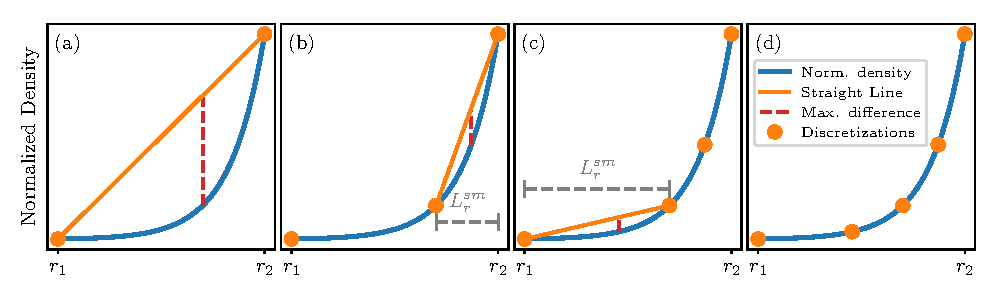
\includegraphics[width=\linewidth]
    {figures/density-based-discretization-algorithm.pdf}
\caption{
    Example application of the density-based discretization algorithm to a non-linear
    density function.
    (a) The normalised density function $\rho_n(r')$ (blue), current boundaries of the
    tesseroid (orange dots), and the linear density function $\rho_l(r')$ (orange line).
    The dashed red line represents the maximum density difference $\Delta \rho (r')$ at
    which the tesseroid would be divided (assuming that the
    inequality~\ref{eq:delta-density} is not satisfied).
    (b) Second iteration of the algorithm with a new linear density function and maximum
    density difference. The tesseroid would be divided at the depth indicated by the
    dashed red line.
    (c) Third iteration of the algorithm.
    (d) Final output of the density-based discretization, assuming that all four new
    tesseroids satisfy inequality~\ref{eq:delta-density}.
}
\label{fig:density-discretization-algorithm}
\end{figure*}

The numerical integration of an arbitrary continuous density function introduces a new
type of problem: the integration error from using only a few nodes to account for the
variation of the density function.
The three dimensional adaptive discretization may help
to reduce this kind of error by adding more point masses in the radial direction.
However, it does not take into account the density function when subdividing the
tesseroid and hence it is not well suited to fully perform this task.
The two dimensional adaptive discretization algorithm does not subdivide the tesseroid
on the radial dimension, so it does not put any effort on lowering this new kind of
error.

We have developed a complementary discretization
algorithm that takes into account the variations of the density function.
This density-based discretization is applied prior to the adaptive discretization
described in the previous section.
In short, the algorithm divides the tesseroid along the radial dimension at the
depths at which the \emph{maximum density variations} take place.

Consider an \emph{original} tesseroid with a continuous density given by the function
$\rho(r')$.
Before the density-based discretization starts,
we normalise the density function to the range $[0, 1]$ as follows

\begin{equation}
    \rho_n(r') =
    \frac{\rho(r') - \rho_\text{min}}{\rho_\text{max} - \rho_\text{min}},
\end{equation}

\noindent in which $\rho_\text{min}$ and $\rho_\text{max}$ are the minimum and maximum
density values inside the tesseroid boundaries.
We emphasize that this normalised density function will not be modified throughout the
algorithm.
In case the density function is constant, both maximum and minimum densities will be
equal and the density-based discretization algorithm will not be applied.

The algorithm is comprised of the following steps
(Fig.~\ref{fig:density-discretization-algorithm}):

\textit{Step 1}:
Define a linear function $\rho_l(r')$ that assumes
the same values as the normalised density $\rho_n(r')$ at the boundaries of the
tesseroid ($r_1$ and $r_2$):

\begin{equation}
    \rho_l(r') =
    \frac{ \rho_n(r_2) - \rho_n(r_1) }{ r_2 - r_1 } (r' - r_1) + \rho_n(r_1),
    \label{eq:density-reference-line}
\end{equation}

\textit{Step 2}:
Evaluate the normalized and linear density functions on a range of $N$ radii between
$r_1$ and $r_2$.
We have opted for $N = 101$ but the specific value of $N$ is not critical to the
algorithm.

\textit{Step 3}:
Compute the absolute difference between the values of the linear and normalised density
functions:

\begin{equation}
    \Delta \rho (r') = | \rho_n(r') - \rho_l(r') |.
    \label{eq:density-abs-diff}
\end{equation}

\textit{Step 4}:
If the following inequality holds, the tesseroid will not be divided:

\begin{equation}
    \text{max}\{ \Delta \rho(r') \} \frac{L_r}{L_r^\text{orig}} \le \delta,
    \label{eq:delta-density}
\end{equation}

\noindent
in which $L_r$ is the radial dimension of the tesseroid being considered for division,

\begin{equation}
    L_r = r_2 - r_1,
\end{equation}

\noindent $L_r^\text{orig}$ is the radial dimension of the original tesseroid, and
$\delta$ is a positive constant henceforth called the \textit{delta ratio}.

\textit{Step 5}:
If inequality~\ref{eq:delta-density} is not satisfied, then the tesseroid is split in
two parts at the radius $r_\text{max}$ at which the maximum absolute difference
(Eq.~\ref{eq:density-abs-diff}) takes place.

\textit{Step 6}:
Repeat steps 1-6 for each smaller tesseroid produced in step 5.

Once all smaller tesseroids satisfy Eq.~\ref{eq:delta-density},
each one is subjected to the two dimensional adaptive
discretization algorithm described earlier to calculate their gravitational effects.

On the first iteration, the ratio $L_r/L_r^\text{orig} = 1$ because the tesseroid being
divided is the original one.
For further iterations, the ratio will be progressively smaller than one as the
tesseroids get smaller.
This is intended to limit the number of divisions to the ones that will
significantly reduce the numerical error:
dividing a large tesseroid with a small $\text{max}\{ \Delta \rho(r') \}$ would
improve the integration accuracy more than dividing a small tesseroid with a
higher $\text{max}\{ \Delta \rho(r') \}$.

The higher $\delta$ is, the fewer divisions will be made, and vice-versa.
Thus, it controls how many times the tesseroids will be divided based on the density
function and, indirectly, determines the accuracy and computation time of
numerical integration.
This raises the need to determine a maximum value of $\delta$ that
ensures an acceptable accuracy while minimising the computation time.


\subsection{Algorithm summary}

In summary, given any tesseroid with variable density in depth and an arbitrary
external computation point, we propose the following steps to numerically
compute the gravitational fields:

\textit{Step 1:}
Apply the density-based discretization algorithm.
It subdivides the tesseroid only in the radial dimension, thus it will return a set of
tesseroids with the same longitudinal and latitudinal dimensions as the original one but
with different radial boundaries.

\textit{Step 2:}
Apply the two dimensional adaptive discretization algorithm on each tesseroid obtained
in the previous step.
If needed, it will subdivide each tesseroid only in the latitudinal and longitudinal
direction, generating a set of smaller tesseroids that resemble the original one.

\textit{Step 3:}
Apply a second-order GLQ to numerically compute the gravitational fields
(Eq.\ref{eq:glq-var-dens}) generated by each tesseroid obtained in the
previous step.
Then sum these results in order to obtain the gravitational field of the original
tesseroid.


\subsection{Software implementation}

We have implemented the algorithms described in the previous sections in the Python
programming language.
The software is based on the pre-existing code for the homogeneous density tesseroid
\citep{Uieda2016}, more specifically the implementation in the Python library Fatiando a
Terra v0.5 \citep{Uieda2013}.
The more time consuming parts of the algorithm are written in the Cython language to
achieve higher performance.
This new code is freely available under the BSD 3-clause open-source license.
It can be downloaded from the online repository
\href{https://github.com/pinga-lab/tesseroid-variable-density}{github.com/pinga-lab/tesseroid-variable-density}.



%%%%%%%%%%%%%%%%%%%%%%%%%%%%%%%%%%%%%%%%%%%%%%%%%%%%%%%%%%%%%%%%%%%%%%%%%%%%%

\section{Determination of the distance-size and delta ratios}

The distance-size ratio $D$ of the adaptive discretization and the delta ratio $\delta$
of the density-based discretization determine how many times each tesseroid will be
divided and thus indirectly control the numerical error of the integration.
Optimal values for $D$ and $\delta$ must be determined in order to ensure both
acceptable numerical accuracy and computation efficiency for the algorithm.

\citet{Uieda2016} compared the numerical integration of homogeneous density tesseroids
with the analytical solution of a spherical shell \citep{Mikuska2006, Grombein2013} in
order to obtain default values for the distance-size ratio $D$.
We will follow this idea but for our needs the spherical shell must
have the same density function of radius as our tesseroid model.
\citet{Lin2018} show the analytical solution of the gravitational potential generated by
a spherical shell with linear density in the radial coordinate.
We derive an expression for such gravitational potential in case the spherical shell has
an arbitrary density function in depth (Eq.~\ref{eq:shell-pot}), and obtained the
expressions in case of linear and exponential density (see Appendix~\ref{sec:shell}).

We perform comparisons between the analytical solutions for the spherical shell and the
numerical integration results for linear, exponential and trigonometric density
functions.
From these results, we generalize default values for $D$ and $\delta$ that ensure a
numerical error lower than 0.1\% of the spherical shell values.

\begin{table}
\caption{
    Description of the tesseroid models used to build spherical shells and characterize
    the accuracy of the numerical integration.
    The first column indicates the thickness of the shell model and the next three
    describe the shape of the tesseroid model: each one specifies the number of
    tesseroids on the corresponding dimension (radial, latitudinal, longitudinal).
    The last two columns specify the latitudinal and longitudinal size of each
    tesseroid that compose the spherical shell model.
    The outer radius of every shell model is equal to the mean Earth radius (6378.137
    km), while the inner radius is determined by its thickness.
}
\label{tab:shell-models}
\begin{tabular}{cccccc}
    Thickness & Radial & Latitudinal & Longitudinal & $L_\phi$ & $L_\lambda$ \\ \hline
    100m   & 1 & 6 & 12 & 30$^\circ$ & 30$^\circ$ \\
    1km    & 1 & 6 & 12 & 30$^\circ$ & 30$^\circ$ \\
    10km   & 1 & 6 & 12 & 30$^\circ$ & 30$^\circ$ \\
    100km  & 1 & 6 & 12 & 30$^\circ$ & 30$^\circ$ \\
    1000km & 1 & 6 & 12 & 30$^\circ$ & 30$^\circ$ \\
\end{tabular}
\end{table}

\begin{table}
\caption{
    Description of the computation grids used to characterize the accuracy of the
    numerical integration.
    Grid height is defined above the mean Earth radius.
}
\label{tab:grids}
\begin{tabular}{lccc}
    Name & Grid size & Grid region (degrees) & Grid height (km)
    \\ \hline
    Pole      & $0.1^\circ \times 0.1^\circ$ &   0E /   1E / 89N / 90N & 0   \\
    Equator   & $0.1^\circ \times 0.1^\circ$ &   0E /   1E /  0N / 1N  & 0   \\
    Global    & $ 10^\circ \times  10^\circ$ & 180W / 180E / 90S / 90N & 0   \\
    Satellite & $ 10^\circ \times  10^\circ$ & 180W / 180E / 90S / 90N & 260 \\
\end{tabular}
\end{table}


\subsection{Linear Density}

A spherical shell with a linear density function given by

\begin{equation}
    \rho(r') = ar' + b,
    \label{eq:density-linear}
\end{equation}

\noindent
has an analytical solution given by Eq.~\ref{eq:shell-pot-linear}.

The absolute density difference defined on equation~\ref{eq:density-abs-diff} will
always be zero for the linear density case.
As a result, the inequality~\ref{eq:delta-density} will always be satisfied and no
divisions will ever be performed.
Therefore, the two dimensional adaptive discretization algorithm is the
only mechanism that controls the accuracy of the numerical integration.
For this reason, we will only determine the minimum value of $D$ needed in order to
guarantee an acceptable accuracy while ignoring the value of $\delta$.

In order to compare the numerical results with the analytical solution we must build
spherical shell models made of tesseroids: we choose to regularly split the spherical
shell along the latitudinal and longitudinal directions obtaining a shell model made out
of $30^\circ \times 30^\circ$ tesseroids.
In order to cover different computation scenarios we use five spherical shells, each one
with the outer radius equal to the mean Earth radius and the inner radius determined by
the desired thickness (100m, 1km, 10km, 100km and 1000km).
These shell models are detailed on Table~\ref{tab:shell-models}.

The comparison between the numerical results and the analytical solution could be
naively compared on a single computation point due to the rotation symmetry of the
spherical shell.
But the numerical results may adopt different values depending on the relative location
between the computation point and the tesseroid, thus is not wise to carry out the
comparison on a single point.
Instead, we propose four computation grids detailed on Table~\ref{tab:grids}: a Pole and
an Equator grids, and a Global and Satellite grids.
The former ones are regional scale grids located on the outer surface of the spherical
shell, while the latter are global scale grids located at zero height (Global) and at
the mean orbital height of the gravimetric satellite missions (Satellite).
We define these grids in the spirit of spanning a broad scenario of gravitational field
computations and ensure an acceptable accuracy on each one of them.
The comparison will be carried out by computing the maximum absolute difference between
the analytical solution and the numerical result on each point of the computation grid.

We assign a density that varies linearly with $r$ (Eq.~\ref{eq:density-linear}) to each
shell model, which assumes the values of $\rho_\text{in} = 3300$~kg/m$^3$ and
$\rho_\text{out} = 2670$~kg/m$^3$ on the inner and outer radii, respectively.
So, the constants $a$ and $b$ from Eq.~\ref{eq:density-linear} must be

\begin{equation}
    a = \frac{\rho_\text{out} - \rho_\text{in}}{R_\text{out} - R_\text{in}},
\end{equation}

\begin{equation}
    b = \rho_\text{out} -
    \frac{\rho_\text{out} - \rho_\text{in}}{R_\text{out} - R_\text{in}} R_\text{out},
\end{equation}

\noindent
where $R_\text{out}$ and $R_\text{in}$ are the outer and inner radii of the shell,
respectively.
Because the outer radius of every spherical shell model will be equal to the mean Earth
radius, $R_\text{out} = 6378.137 \text{km}$.

\begin{figure*}
\centering
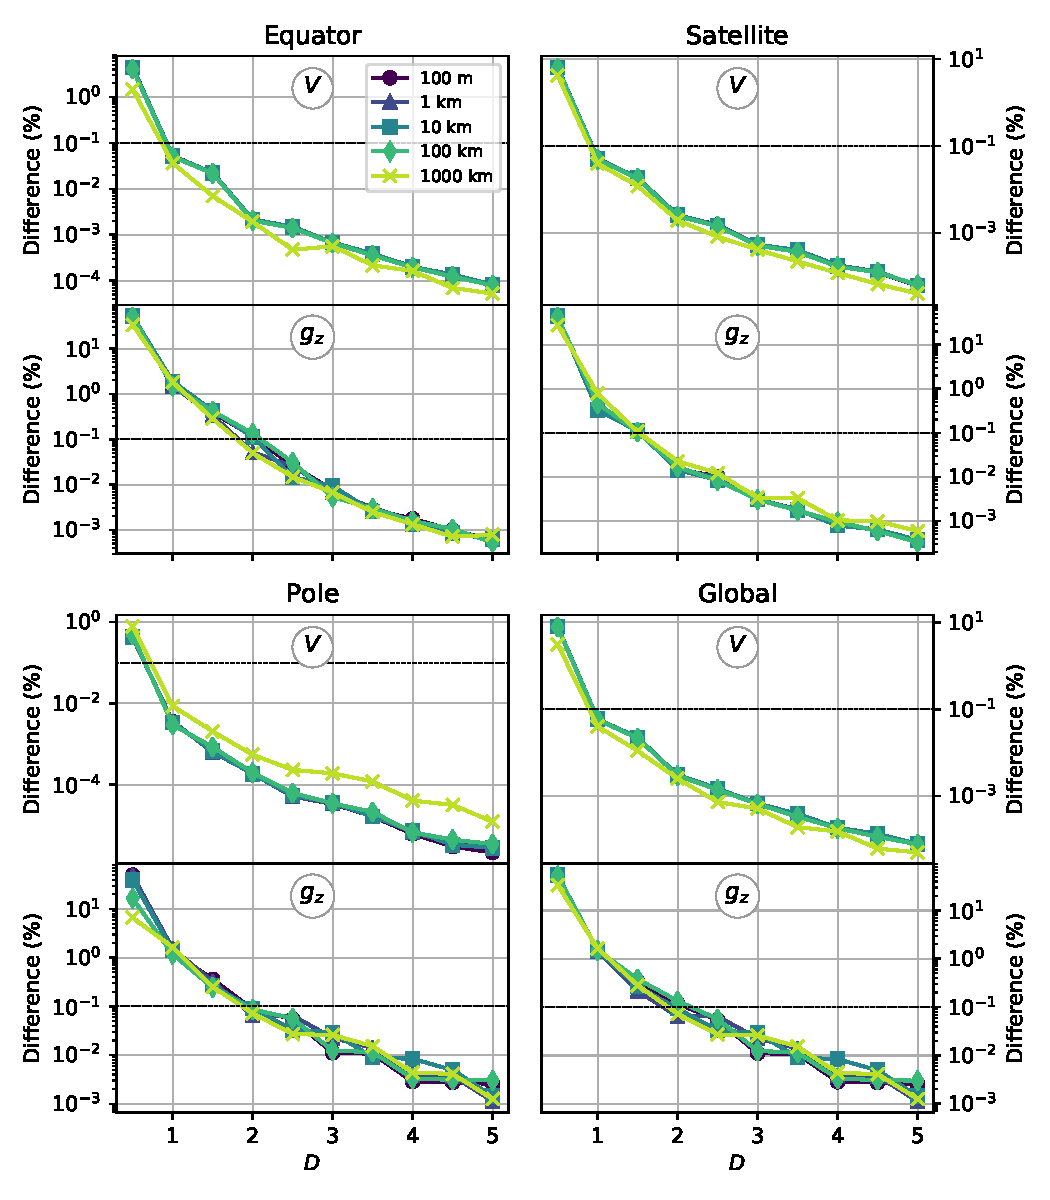
\includegraphics[width=\linewidth]{figures/linear-density-diffs.pdf}
\caption{
    Differences between the gravitational fields generated by each tesseroid shell model
    and the analytical solution.
    Each model has a linear density function (Eq.~\ref{eq:density-linear}).
    The computations were performed on the four grids described in Table~\ref{tab:grids}
    and using the shell models detailed in Table~\ref{tab:shell-models}.
    Each line represents the maximum absolute difference between every shell model.
    Due to the linearity of the density function, the density-based discretization
    algorithm is not applied.
    Differences are reported as a percentage of the shell values.
    The horizontal dashed black line represents a target difference of 0.1\%.
}
\label{fig:D-linear}
\end{figure*}

We compute the gravitational potential ($V$) and the vertical component of the gradient
($g_z$) that each shell model generates on each computation grid.
Other components of the gradient are equal to zero outside of the shell due to the
rotational symmetry and are thus omitted from the analysis.
The computations are repeated for values of $D$ ranging from 0.5 to 5 with a step of
0.5.
Then we calculate the absolute difference between these results and the analytical
solution, taking only the maximum absolute difference on each computation grid.
This differences are shown in Fig.~\ref{fig:D-linear}.
Finally, we set the optimal value of $D$ as the minimum value at which the corresponding
error of the numerical approximation is lower than 0.1\%.

We observe from Fig.~\ref{fig:D-linear} that the relative errors for the
potential and the $g_z$ component fall below the 0.1\% threshold at
$D=1$ and $D=2.5$, respectively, for every shell model and computation grid.
These results also show that there's no meaningful dependency between the accuracy of
the method and the thickness of the shell or the height of the computation grid (the
results for the Satellite grid and the Global grid are very similar).


\subsection{Exponential Density}

For an exponential density function, the density-based discretization will be applied
before the adaptive discretization algorithm.
This means that optimal values for both the distance-size ratio $D$ and the delta ratio
$\delta$ must be determined.
We perform an error analysis similar to what was done for the linear density case.
But, now the spherical shell will have an exponential density function that assumes the
values of $\rho_\text{out} = 2670$~kg/m$^3$ and $\rho_\text{in} = 3300$~kg/m$^3$ on the
outer and inner surfaces, respectively, defined as follows:

\begin{equation}
    \rho(r') = A e^{- \frac{b}{T} (r' - R_1)} + C,
    \label{eq:density-exp}
\end{equation}

\noindent where

\begin{equation}
    A = \frac{\rho_\text{in} - \rho_\text{out}}{1 - e^{-b}},
\end{equation}

\begin{equation}
    C = \rho_\text{in} - A,
\end{equation}

\noindent $T$ is the thickness of the shell ($T = R_2 - R_1$) and $b$ is a dimensionless
constant that determines the variability of the function: a higher value of $b$
increases the maximum slope of the density function.
On exponential density analysis we will use values of $b$ equal to 1, 2, 5, 10, 30
and 100, in order to cover different kind of exponential density variations, from smooth
to sharp (Fig.~\ref{fig:exp-densities}).

\begin{figure}
\centering
\iftwocol{
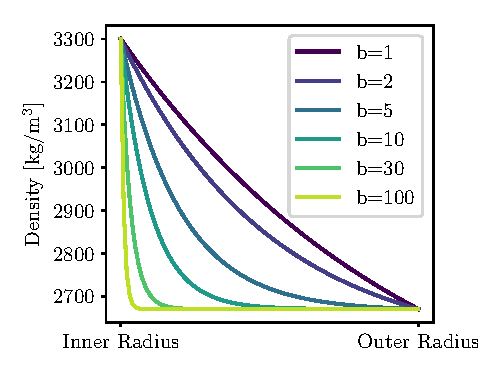
\includegraphics[width=\linewidth]{figures/exponential-densities.pdf}
}{
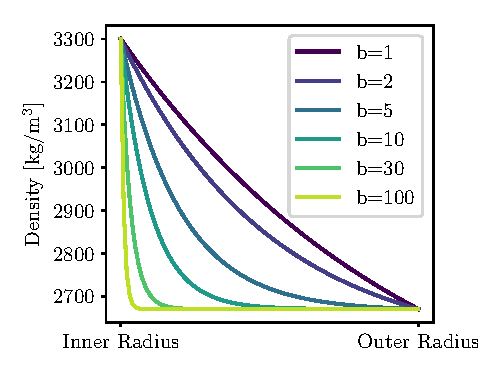
\includegraphics[width=0.5\linewidth]{figures/exponential-densities.pdf}
}
\caption{
    Exponential density functions assigned to each spherical shell in the $D$ and
    $\delta$ ratios determination.
    Each density function corresponds to a different value of $b$ on
    Eq.~\ref{eq:density-exp}.
}
\label{fig:exp-densities}
\end{figure}


\subsubsection{$D$-$\delta$ space exploration}

We aim to find a combination of the $D$ and $\delta$ that produces a numerical error
lower than the 0.1\% threshold while minimizing computation time.
We use a grid search method and compute the numerical error for every ($D$, $\delta$)
pair belonging to a grid on the $D$-$\delta$ space (Fig.~\ref{fig:grid-search}).
For optimum algorithm performance, we search for the ($D$, $\delta$) pair that minimize
the number of splittings while keeping a numerical error under the 0.1\% threshold,
i.e.~the smallest possible value of $D$ and the highest possible value of $\delta$.

We compute the relative difference between the numerical and analytical results for the
gravitational potential ($V$) and the vertical component of its gradient ($g_z$) on the
computation grids detailed in Table~\ref{tab:grids}.
Because this is a time consuming computation, we limit the analysis only to a single
value of $b$ equal to 30 (Fig.~\ref{fig:exp-densities}).
For the sake of brevity, we compute the maximum differences between the results for each
shell model.
The results are shown in Fig.~\ref{fig:grid-search}, in which points inside the dotted
lines are the ones that present a numerical error lower than the 0.1\% threshold.
Also shown in Fig.~\ref{fig:grid-search} are the $D$ values determined for the linear
density function in the previous section ($D_\text{linear}$).

The minimum values of $D$ that are within the 0.1\% threshold are the $D_\text{linear}$
ones, i.e.~they are the optimal values of the distance-size ratios for $V$ and $g_z$.
These results indicate that the values of $D_\text{linear}$ can be safely extrapolated
to the exponential case.
This conclusion can be understood considering that the two dimensional adaptive
discretization and the density-based algorithms are independent of each other: the first
one splits the tesseroid only in the latitudinal and longitudinal directions, while the
latter only does it in the radial direction.
This leads to the fact that the value of $\delta$ needed to limit the numerical error
due to the density variation is independent of the value of $D$ and vice versa.
That's why the optimal distance-size ratios for the exponential density case is the same
as the ones for the linear density case.

Because the grid search was limited to specific values of $b$ and used only one grid, we
will perform a more detailed analysis for $\delta$ determination in case of exponential
density tesseroids.

\begin{figure}
\centering
\iftwocol{
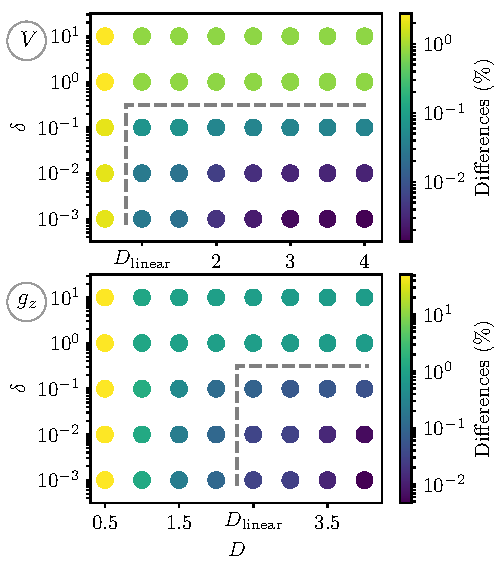
\includegraphics[width=\linewidth]
    {figures/grid-search.pdf}
}{
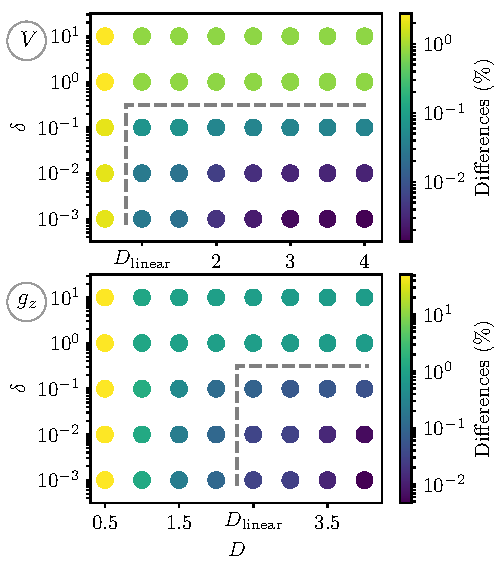
\includegraphics[width=0.5\linewidth]
    {figures/grid-search.pdf}
}
\caption{
    Numerical error exploration in the $D$-$\delta$ space.
    The percentage difference values were obtained from the comparison between the
    analytical solution and the numerical approximation of the gravitational fields ($V$
    and $g_z$) generated by a spherical shell with an exponential density function
    (Eq.~\ref{eq:density-exp}).
    These comparisons were carried out on the ``Global'' grid (Table~\ref{tab:grids}),
    with the spherical shell models detailed in Table~\ref{tab:shell-models}, and an
    exponential density function with $b = 30$.
    The percentage difference values are obtained as the maximum difference
    between every shell model.
    The points inside the dashed line are the ones that present an error lower than
    0.1\%.
    The $D$ value obtained for the linear density case for each gravitational field is
    also shown ($D_\text{linear}$).
    }
\label{fig:grid-search}
\end{figure}


\subsubsection{Delta ratio determination}

\begin{figure*}
\centering
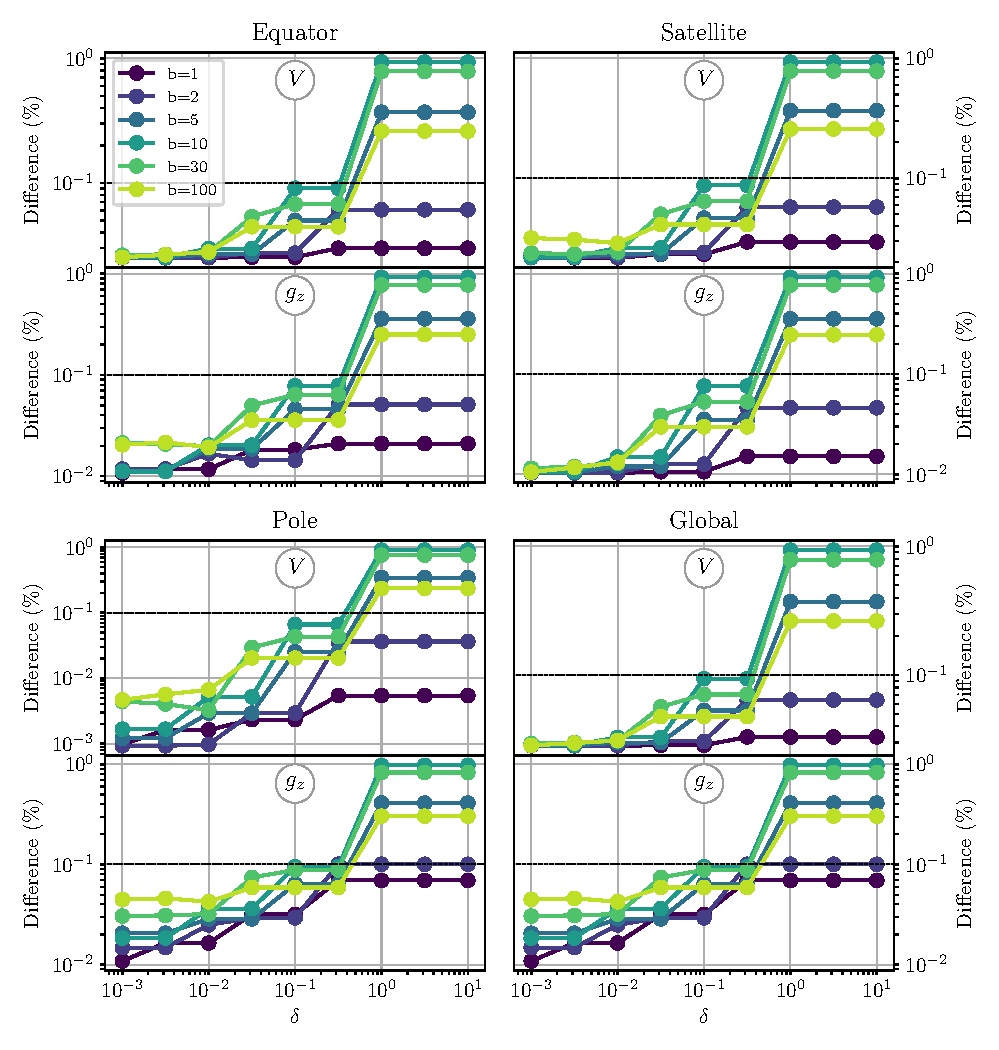
\includegraphics[width=\linewidth]{figures/exponential-density-diffs.pdf}
\caption{
    Numerical error for different exponential density functions and values of the delta
    ratio.
    The percentage difference values were obtained from the comparison between the
    analytical solution and the numerical approximation of the gravitational fields ($V$
    and $g_z$) generated by the spherical shell with an exponential density function and
    different values of $b$ (Eq.~\ref{eq:density-exp}).
    These comparisons were carried out on every grid defined on Table~\ref{tab:grids},
    making use of the shell models detailed on Table~\ref{tab:shell-models} and
    fixing the distance-size ratio $D$ to the values obtained for the linear density
    case.
    Each curve corresponds to the maximum difference between every shell model with the
    same value of $b$.
    }
\label{fig:delta-exponential}
\end{figure*}

Having chosen values of $D$ equal to the ones obtained for the linear density case, we
are free to explore the integration error as a function of $\delta$ in more detail and
how it varies for different values of $b$ (Eq.~\ref{eq:density-exp}).
Now we perform the error calculations for values of delta ranging from $10^{-3}$ to
$10^{1}$, for every grid detailed in Table~\ref{tab:grids} and for the spherical shell
models detailed in Table~\ref{tab:shell-models}.
The calculations are repeated for distinct values of $b$ (1, 2, 5, 10, 30, 100) to
examine the accuracy of the method for different sharpness of the density function.
Because larger $\delta$ values result in fewer tesseroid divisions,
our intention is to find the highest value of $\delta$ whose numerical error is bellow
the $0.1\%$ threshold.

Fig.~\ref{fig:exp-densities} shows the density functions for each value of $b$ and
Fig.~\ref{fig:delta-exponential} shows the resulting relative
differences ($V$ and $g_z$).
In order to improve the visualization of the results, each curve corresponds to the
maximum difference between all shell models for the same value of $b$.
The relative difference for $V$ and $g_z$ falls below the 0.1\% threshold
for each computation grid, shell model and $b$ value if $\delta = 0.1$.
This results imply that a value of $\delta=0.1$ is needed in order to
achieve the 0.1\% accuracy threshold for both the potential and the $g_{z}$, every
shell model, computation grid and value of $b$, in case of exponential density.
These results also show that there is no significant relation between the $b$
value and the numerical error, proving that the density-based discretization algorithm
is capable of limiting the error due to the density variation regardless the variation
of the exponential density.


\subsection{Sinusoidal Density}

So far we have tested the density-based discretization algorithm against linear and
exponential density functions.
Nevertheless, this new algorithm is well suited to accurately reproduce the
gravitational fields of tesseroids with more complex continuous functions, like
non-monotonic or with one or more inflection points.
Although such density functions are very rare (or maybe even non-existent) between
geological structures, we want to subject the density-based algorithm to such cases in
order to show that it can solve more complex situations other than linear and
exponential functions.

We will consider spherical shells with a sinusoidal density defined as follows:

\begin{equation}
    \rho(r') = A \sin \left( 2 \pi b \frac{r' - R}{T} \right) + A,
    \label{eq:density-sine}
\end{equation}

\noindent where $A$ is a constant, $T$ is the thickness of the shell, $R$ is the mean
Earth radius and $b$ is a dimensionless constant that regulates how many periods of the
trigonometric function are included inside the inner and outer radii.
For this analysis we will use values of $b$ equal to 1, 2, 5 and 10
(Fig.~\ref{fig:sine-densities}).
We shift the sine function in order to prevent near zero values of the potential and the
$g_z$.

We compute the relative difference between the numerical and analytical results for the
gravitational potential ($V$) and the $g_z$ of the spherical shells detailed in
Table~\ref{tab:shell-models} on each grid detailed in Table~\ref{tab:grids}.
Each shell is assigned with different sinusoidal density functions by changing the
values of $b$ in Eq.~\ref{eq:density-sine} (Fig.~\ref{fig:sine-densities}).
The analytical solution for the potential $V$ can be found on Appendix~\ref{sec:shell}.
We fixed the distance-size ratio $D$ to the ones obtained for the linear density case
and explored values of $\delta$ ranging from $10^{-4}$ to $1$.

\begin{figure}
\centering
\iftwocol{
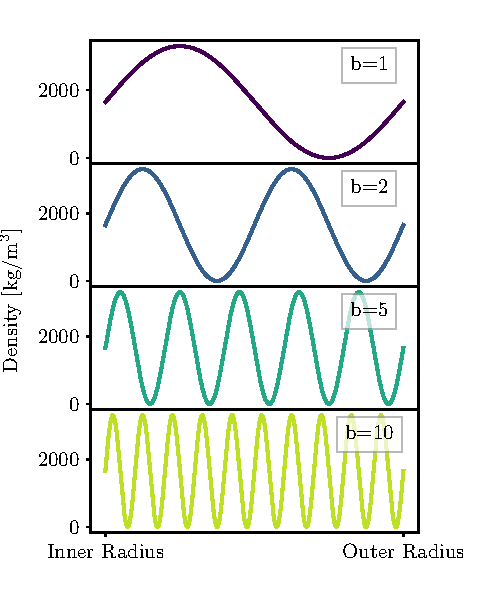
\includegraphics[width=\linewidth]{figures/sine-densities.pdf}
}{
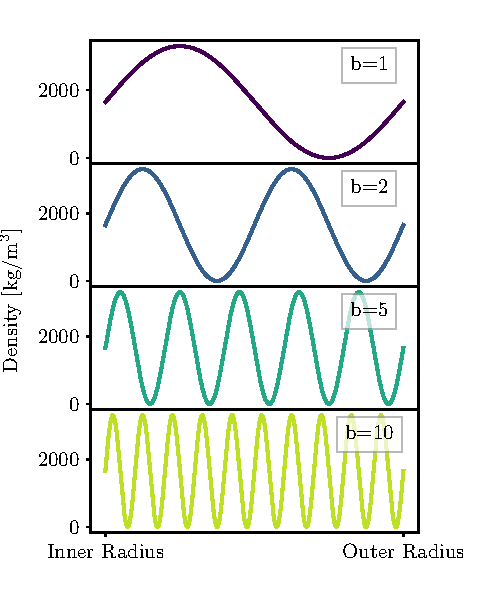
\includegraphics[width=0.5\linewidth]{figures/sine-densities.pdf}
}
\caption{
    Sinusoidal density functions assigned to each spherical shell in the $\delta$ ratio
    determination.
    Each density function corresponds to a different value of $b$ on
    Eq.~\ref{eq:density-sine}.
}
\label{fig:sine-densities}
\end{figure}

\begin{figure*}
\centering
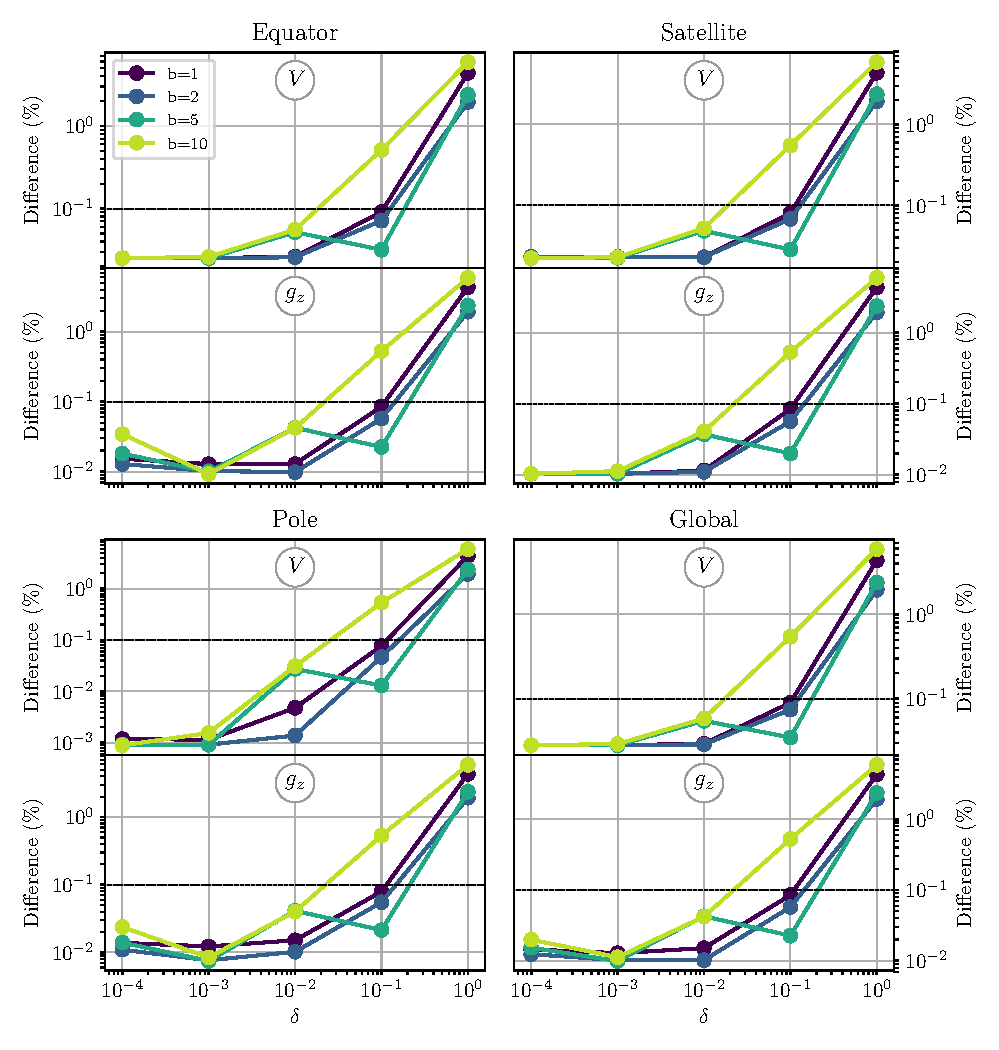
\includegraphics[width=\linewidth]{figures/sine-density-diffs.pdf}
\caption{
    Numerical error for different sinusoidal density functions and values of the delta
    ratio.
    The percentage difference values were obtained from the comparison between the
    analytical solution and the numerical approximation of the gravitational fields ($V$
    and $g_z$) generated by the spherical shell with an exponential density function and
    different values of $b$ (Eq.~\ref{eq:density-sine}).
    These comparisons were carried out on every grid defined on Table~\ref{tab:grids},
    making use of the shell models detailed on Table~\ref{tab:shell-models} and
    fixing the distance-size ratio $D$ to the values obtained for the linear density
    case.
    Each curve corresponds to the maximum difference between every shell model with the
    same value of $b$.
    }
\label{fig:delta-sine}
\end{figure*}

Fig.~\ref{fig:sine-densities} shows the sinusoidal density functions assigned to every
spherical shell and Fig.~\ref{fig:delta-sine} shows the resulting relative differences
between the analytical and the numerical solutions.
In order to improve the visualization of the results, each curve corresponds to the
maximum difference between all shell models for the same value of $b$.
For this kind of sinusoidal density, a value of $\delta=0.01$ is needed in order to
achieve the 0.1\% accuracy threshold for both the potential and the $g_{z}$, every
shell model, computation grid and value of $b$.
This results also proof that even for a continuous density function with several local
maximum and minimums and inflection points, the density-based discretization algorithm
performs well on computing the gravitational fields that a tesseroid with such density
generates.


%%%%%%%%%%%%%%%%%%%%%%%%%%%%%%%%%%%%%%%%%%%%%%%%%%%%%%%%%%%%%%%%%%%%%%%%%%%%%%%

\section{Computation time comparison}

Because the density-based algorithm produces discretizations along the radial direction,
besides the latitudinal and longitudinal ones generated by the two dimensional adaptive
one, the computation time of the gravitational fields of variable density tesseroids
will be increased in comparison to the homogeneous density case.
In order to quantize this increase we perform a computation time comparison between the
homogeneous density case with the linear and the exponential ones.

We define a $20^\circ \times 20^\circ$ tesseroid of 1km of thickness and a single
computation point located at different heights (1m, 10m, 100m, 1km, 10km, 100km and
1000km) above the top surface of the tesseroid.
Then we compute the gravitational potential $V$ and the $g_z$ that the tesseroid
generates on the computation point in case of an homogeneous density, a linear density
and an exponential density with $b = 3$ (Eq.~\ref{eq:density-exp}).
We perform 1000 computations for each field, density and computation height while
tracking the computation time for each one of them.
The final computation time is obtained as the mean value of these runs.

Fig.~\ref{fig:computation-times} shows the computation time ratio between the
computations times of the linear and exponential density with the one for an homogeneous
density, defined as:

\begin{equation}
    \text{Computation time ratio} = \frac{\Delta t}{\Delta t_\text{homog}},
\end{equation}

\noindent where $\Delta t_\text{homog}$ is the computation time for the homogeneous
density and $\Delta t$ is the computation time for the linear or the exponential
density.

\begin{figure}
\centering
\iftwocol{
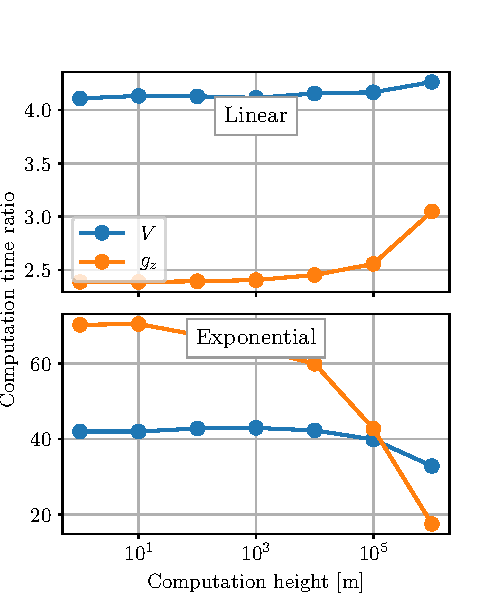
\includegraphics[width=\linewidth]{figures/computation-times.pdf}
}{
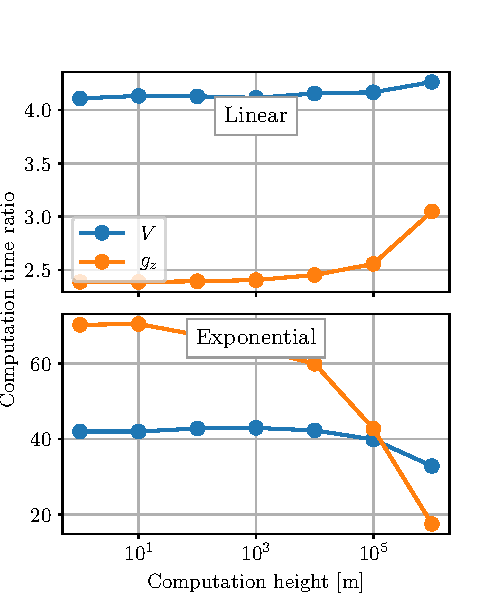
\includegraphics[width=0.5\linewidth]{figures/computation-times.pdf}
}
\caption{
    Computation times ratio between linear and exponential density tesseroids with an
    homogeneous one.
}
\label{fig:computation-times}
\end{figure}


%%%%%%%%%%%%%%%%%%%%%%%%%%%%%%%%%%%%%%%%%%%%%%%%%%%%%%%%%%%%%%%%%%%%%%%%%%%%%%%

\section{Application to the Neuqu\'en Basin}

We applied the new algorithms and optimal values of $D$ and $\delta$ determined
previously to calculate the gravitational effects of the Neuqu\'en Basin:
a sedimentary basin
located to the east of the Andes, between 32$^\circ$S and 40$^\circ$S latitude
(Fig.~\ref{fig:neuquen-basin}a).
The basin includes continental and marine siliciclastics, carbonates, and evaporites
accumulated over the Jurassic and the Cretaceous constituting a stratigraphic record up
to 5000m of depth \citep{Howell2005}.

\begin{figure}
\centering
\iftwocol{
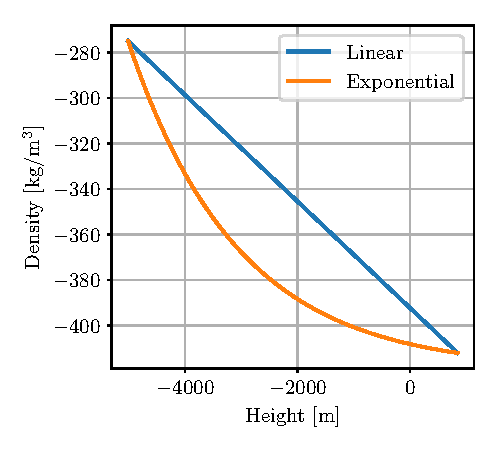
\includegraphics[width=\linewidth]{figures/neuquen-basin-densities.pdf}
}{
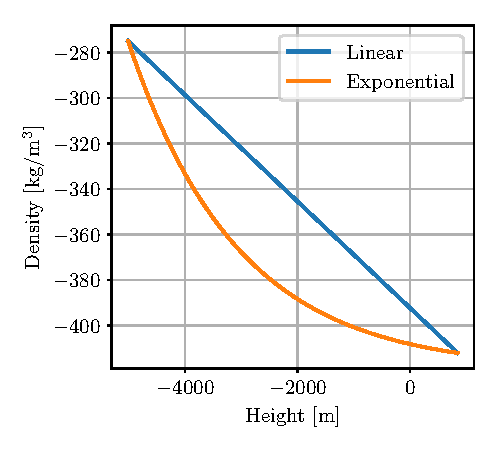
\includegraphics[width=0.5\linewidth]{figures/neuquen-basin-densities.pdf}
}
\caption{
    Linear and exponential densities used to compute the gravitational fields generated
    by a tesseroid model of the Neuquen sedimentary basin.
    The height is defined above the mean Earth radius, and its axis is spanned between
    the deepest and the highest point of the basin.
}
\label{fig:neuquen-basin-densities}
\end{figure}

\begin{figure*}
\centering
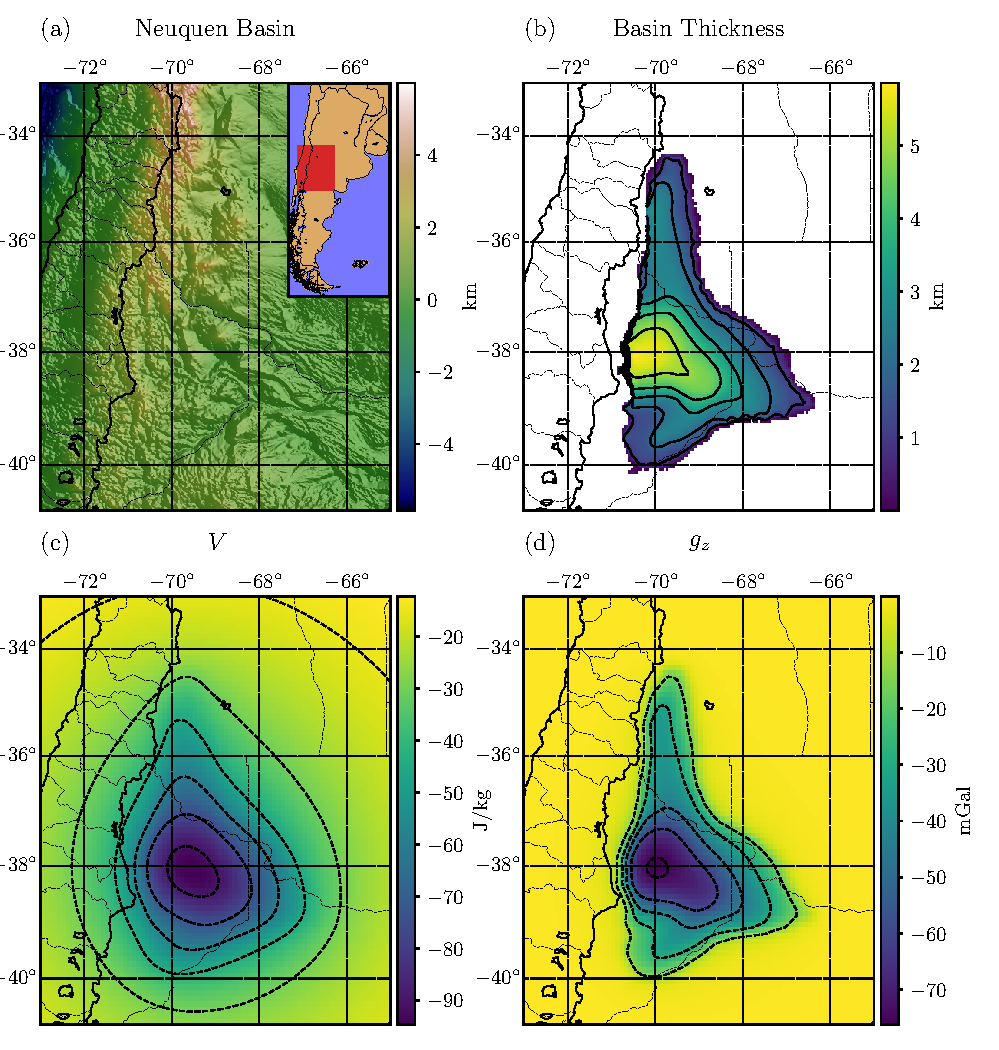
\includegraphics[width=\linewidth]{figures/neuquen-basin.pdf}
\caption{
    Gravitational effects of the Nequ\'en sedimentary basin modelled
    using tesseroids with an exponential density function of depth.
    (a) Topography of the Neuqu\'en Basin (in km) and its location in South America,
    (b) thickness of the sedimentary basin \citep[in meters;][]{Heine2007},
    (c) resulting gravitational potential $V$,
    (d) resulting vertical component of the gradient ($g_z$),
    calculated at 10km of height over the mean Earth radius.
}
\label{fig:neuquen-basin}
\end{figure*}

\begin{figure*}
\centering
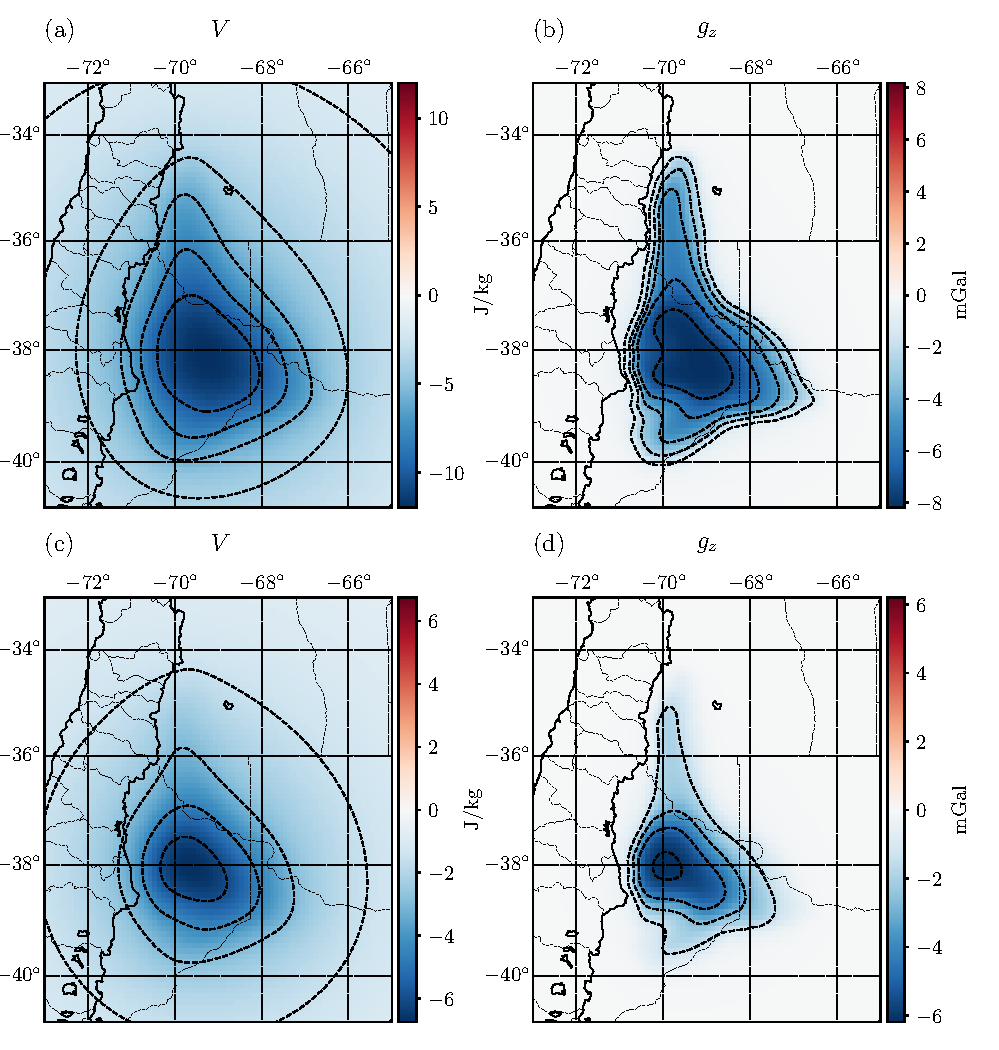
\includegraphics[width=\linewidth]{figures/neuquen-basin-diffs.pdf}
\caption{
    Differences between the gravitational fields generated by the tesseroid model of the
    Neuquen basin with an exponential density contrast and with a homogenenous and
    linear density variation.
    (a)-(b) Differences on $V$ and $g_z$ between the exponential density model and the
    homogenenous density one,
    (c)-(f) differences on $V$ and $g_z$ between the exponential density model and the
    linear density one,
    calculated at 10km of height over the mean Earth radius.
}
\label{fig:neuquen-basin-diffs}
\end{figure*}

The thickness of the sediment pack was digitized from \citet{Heine2007} on a regular
grid with a resolution of 0.05$^\circ$ on both longitude and latitude directions
(Fig.~\ref{fig:neuquen-basin}b).
We created a tesseroid model of the sediment pack by placing a
$0.05^\circ \times 0.05^\circ$ tesseroid on each node of the grid.
The top of each tesseroid was fixed at the median of the topography of the basin
(845~m above mean Earth radius) and the bottom at corresponding thickness of the basin.

We must also define a density function for the tesseroid model.
\citet{Sigismondi2012} measured a minimum and maximum density contrast for
the Neuqu\'en basin of -412kg/m$^3$ and -275kg/m$^3$, respectively.
We have chosen an exponential density variation (Eq.~\ref{eq:density-exp}) that assumes
the minimum value on the top surface and the maximum at 5014m depth (the thickest part
of the basin), with a value of $b$ equal to 3.
This density variation is in the order of magnitude of the ones used by
\citet{Cowie1990} and \citet{Cordell1973}.
This density function can be seen on Fig.~\ref{fig:neuquen-basin-densities}.

Finally, we computed the gravitational potential $V$ and the vertical component of the
gradient ($g_z$) on a computation grid of $159\times163$ nodes ($0.05^\circ$ spacing on
both longitude and latitude) at a 10km height over the mean Earth radius.
The resulting fields can be seen in Fig.~\ref{fig:neuquen-basin}c-d.
Moreover, we computed the differences between these fields and the ones generated by the
same model but now with a constant density as the mean value between -412kg/m$^3$ and
-275kg/m$^3$, and a linear density that assumes these two values on the highest and the
deepest point of the basin (Fig.~\ref{fig:neuquen-basin-densities}), respectively.
Fig.~\ref{fig:neuquen-basin-diffs}a-b and Fig.~\ref{fig:neuquen-basin-diffs}c-d show the
differences with the constant and the linear density, respectively.


%%%%%%%%%%%%%%%%%%%%%%%%%%%%%%%%%%%%%%%%%%%%%%%%%%%%%%%%%%%%%%%%%%%%%%%%%%%%%%%

\section{Results and Discussion}

The $D$ and $\delta$ ratios determinations proved that for a linear density case only
the two dimensional adaptive discretization algorithm and a second-order GLQ
approximation is needed to achieve a 0.1\% accuracy of the gravitational potential and
the vertical component of the gradient ($g_z$) by using a $D=$ 1 and 2.5 for each field,
respectively.
Although for non-linear functions the adaptive discretization is not sufficient and the
density-based discretization algorithm must be applied.
The $D$-$\delta$ space exploration showed that the more efficient computation takes
place when the value of $D$ equals to the ones determined in the linear density
scenario, while the value of $\delta$ must be determined for each specific density
variation.
In case of an exponential density, a $\delta$ equal to 0.1 is sufficient to achieve the
0.1\% accuracy threshold, while a $\delta = 0.01$ is needed for a sinusoidal density
function.

This result could be extrapolated: a default value of $\delta = 0.01$ would guarantee an
accuracy of 0.1\% in case of an arbitrary continuous density function.
Nevertheless, we encourage to perform similar accuracy tests in order to proof that this
extrapolation works for the desired density function, specially for more complex
variations than a polynomial or exponential one.

\citet{Lin2018} proposed a combined method to efficiently compute gravitational fields
generated by tesseroids: it uses a GLQ with a two dimensional adaptive discretization
algorithm for near computation points and a Taylor series expansion method for far
computation points.
Because our goal is to build a method that could be applied to any continuous density
function, the Taylor series wouldn't be well suited for this task and therefore we
focused only on a pure GLQ approximation method.
Nevertheless, our method could be easily combined with a Taylor series expansion for
specific density function, i.e.~a linear variation.

Moreover, \citet{Lin2018} show that the combined method can be applied to a linear
density variation by splitting the gravitational field integral in two: one for each
term of the linear function.
Our results show that in case of a linear density variation a single GLQ computation is
sufficient to accurately compute the fields, thus reducing the computation time by half.

\citet{Fukushima2018} propose a generalization of his method to polynomial density
functions.
On the other hand, our method is not bounded to a specific density function.
Nevertheless, the density-based discretization algorithm could be used before applying
the numerical integration developed by \citet{Fukushima2018} assigning a low polynomial
order density to each discretizing tesseroid.
Although this method would involve a computational error due to the approximation of the
density function as a polynomial one, it's feasibly if we account for this error and
a method to limit it.

We have also carried out $D$ and $\delta$ determinations for the vertical component of
the Marussi tensor ($g_{zz}$) for linear and exponential densities.
We didn't include these results because our methodology wouldn't achieve the 0.1\%
accuracy threshold for the general case of such density functions.
Moreover, the values of $D$ and $\delta$ needed for the cases at which the accuracy was
below 0.1\% implied a high number of discretizations, thus greatly increasing the
computation time.
In summary, we found the computation of the Marussi tensor components in case of
variable density tesseroids a subject for future research.

%%%%%%%%%%%%%%%%%%%%%%%%%%%%%%%%%%%%%%%%%%%%%%%%%%%%%%%%%%%%%%%%%%%%%%%%%%%%%%%

\section{Conclusions}

We have developed a new methodology to compute the gravitational fields
generated by a tesseroid with a density given by a continuous function of depth.
It numerically solves the integrals that define the gravitational potential,
its gradient, and the Marussi tensor components through the Gauss-Legendre
Quadrature (GLQ).
The accuracy of the numerical integration is automatically controlled by an adaptive
discretization algorithm and a new density-based discretization algorithm.
The former divides the tesseroid in half if the ratio of the distance to the computation
point and the size of the tesseroid is lower than a predefined distance-size ratio $D$.
This algorithm minimises the integration error when the computation point is close to
the tesseroid.
Nevertheless, the adaptive discretization alone is not sufficient to guarantee the
accuracy of the method in case of tesseroids with variable density.

To overcome this challenge, we have developed a density-based discretization algorithm
that divides the tesseroid on the points at which the maximum variations of the density
function take place.
The density-based discretization is performed before adaptive discretization as a type
of pre-processing step.
The number of divisions performed, and thus the accuracy of the computation, is
controlled by the delta ratio $\delta$.
This new algorithm is intended to minimise the error due to the inability of
the GLQ to produce precise approximations of density functions with sharp variations.

Because there is no direct relation between the values assigned to $D$ and $\delta$ and
the error of the computation, we empirically determined the optimum values for these
parameters.
These values minimize the computational load while maintaining the numerical error below
0.1\% of an analytical solution.
The density functions used to establish the optimum values were a linear and an
exponential function.
The linear function represents the smoothest variation of density and does not require
density-based discretization at all.
We analysed the error for exponential functions ranging from smooth to sharp variations
in depth to test the accuracy of the density-based discretization.
Through this analysis, we have obtained optimal values for the distance-size ratio of
1, 2 and 8 for the potential, its gradient, and the Marussi tensor components,
respectively.
These values are in agreement with previous results for a homogeneous density tesseroid
\citep{Uieda2016}.
The optimum $\delta$ values are 0.2 for the potential and its gradient components, while
a $\delta = 0.01$ must be used for the Marussi tensor components in order to ensure a
0.1\% precision.
A wide range of exponential functions were used to infer these results and they are
conservative estimates, chosen to prioritize accuracy over speed of computations.
Therefore, they can be safely generalized to other common depth-density relations, like
quadratic functions, without loss of accuracy.



%%%%%%%%%%%%%%%%%%%%%%%%%%%%%%%%%%%%%%%%%%%%%%%%%%%%%%%%%%%%%%%%%%%%%%%%%%%%%%%

\section{Acknowledgments}

We are indebted to the developers and maintainers of the open-source software without
which this work would not have been possible.

%%%%%%%%%%%%%%%%%%%%%%%%%%%%%%%%%%%%%%%%%%%%%%%%%%%%%%%%%%%%%%%%%%%%%%%%%%%%%%%

\bibliographystyle{gji}
\bibliography{references}

\appendix

\section{Analytical Solutions for Spherical Shell}
\label{sec:shell}

\begin{figure}
\centering
\includegraphics[width=0.5\linewidth]{figures/spherical-shell.pdf}
\caption{
    Spherical shell with inner and outer radii $R_1$ and $R_2$, respectively.
    The computation point $Q$ is located on the $z$ axis at a distance $r$ from
    the origin of the coordinates system.
    For our purposes we will assume that $Q$ is outside of the shell,
    i.e.~$r > R_2$.
}
\label{fig:spherical-shell}
\end{figure}

Consider a spherical shell with inner radius $R_1$ and outer radius $R_2$,
whose density is a function $\rho(r')$ of the radial coordinate
(Fig.~\ref{fig:spherical-shell}).
The gravitational potential generated by the shell on an arbitrary external
point $Q$ can be written as follows:

\begin{equation}
    V_\text{sh}(\phi, \lambda, r) = G
    \int\limits_0^{2\pi}
    \int\limits_{-\frac{\pi}{2}}^\frac{\pi}{2}
    \int\limits_{R_1}^{R_2}
    \frac{\rho(r')}{\ell} {r'}^2 \cos\phi' \,
    dr' d\phi' d\lambda',
\end{equation}

\noindent where $\ell$ is defined in equation~\ref{eq:ell}.

For $Q$ located along the $z$ axis (i.e., $\phi=90^\circ$) at a distance $r$ from the
origin, equation~\ref{eq:ell} simplifies to:

\begin{equation}
    \ell = \sqrt{r'^2 + r^2 - 2 r r' \sin\phi'}.
\end{equation}

\noindent
Because of the rotational symmetry along the $z$ axis, the integration in $\lambda'$ is
straightforward:

\begin{equation}
    V_\text{sh}(r) = 2\pi G
    \int\limits_{-\frac{\pi}{2}}^\frac{\pi}{2}
    \int\limits_{R_1}^{R_2}
    \frac{\rho(r') {r'}^2 \cos\phi'}{\sqrt{r'^2 + r^2 - 2 r r' \sin\phi'}}
    \, dr' d\phi',
\end{equation}

\noindent
while the integration in $\phi'$ can be performed independently of the density function.
Making use of SymPy \citep{sympy2017}, a Python library for symbolic mathematics, we
obtained the following expression for the potential:

\iftwocol{
\begin{equation}
    \begin{split}
        V_\text{sh}(r) = 2\pi G
        \int\limits_{R_1}^{R_2}
        \Big[ & \sqrt{r^2 + r'^2 + 2rr'} - \\
        & \sqrt{r^2 + r'^2 - 2rr'}
        \Big] \frac{r'\rho(r')}{r} \, dr'.
    \end{split}
\label{eq:shell-pot-sqrts}
\end{equation}
}{
\begin{equation}
    V_\text{sh}(r) = 2\pi G
    \int\limits_{R_1}^{R_2}
    \Big[ \sqrt{r^2 + r'^2 + 2rr'}  -
    \sqrt{r^2 + r'^2 - 2rr'}
    \Big] \frac{r'\rho(r')}{r} \, dr'.
\label{eq:shell-pot-sqrts}
\end{equation}
}

Because the computation point $Q$ is outside of the shell, $r > r'$ and the square roots
in equation~\ref{eq:shell-pot-sqrts} simplify to

\begin{equation}
    \sqrt{r^2 + r'^2 + 2rr'} = |r + r'| = r + r',
\end{equation}

\begin{equation}
    \sqrt{r^2 + r'^2 - 2rr'} = |r - r'| = r - r',
\end{equation}

\noindent which leads to the following expression for the potential:

\begin{equation}
    V_\text{sh}(r) = \frac{4\pi G}{r}
    \int\limits_{R_1}^{R_2} {r'}^2 \rho(r') \, dr'.
\label{eq:shell-pot}
\end{equation}

The gradient of potentials that
depends solely on $r$ have only one non zero components: the vertical
component of the gradient ($g_z$).
Following \citet{Grombein2013}:

\begin{equation}
    g_z(r) = \frac{V_\text{sh}(r)}{r},
\end{equation}

From Eq.~\ref{eq:shell-pot} we can obtain expressions of the gravitational potential for
different density functions.

\subsection{Linear density}

For a linear density function

\begin{equation}
    \rho(r') = ar' + b\ ,
\end{equation}

\noindent
the gravitational potential at any external point is

\begin{equation}
    V_\text{sh}^\text{lin}(r) = \pi G \left[
    a \frac{R_2^4 - R_1^4}{r} +
    b \,\frac{4}{3} \frac{R_2^3 - R_1^3}{r} \right].
    \label{eq:shell-pot-linear}
\end{equation}

\noindent The first term on this equation reproduces the potential generated
by a spherical shell with variable density $\rho(r') = ar'$, while the second
term constitutes the potential generated by a spherical shell with homogeneous
density $\rho = b$ \citep{Mikuska2006,Grombein2013}.

\subsection{Exponential density}

For an exponential density function

\begin{equation}
    \rho(r') = A e^{- k (r' - R)},
\end{equation}

\noindent
where $A$, $k$ and $R$ are constants, the gravitational potential on any external point
is

\begin{equation}
    \begin{split}
    V_\text{exp}(r) = \frac{4\pi G}{r} \frac{A}{k^3} \Big[
    & \left( R_1^2 k^2 + 2 R_1 k + 2 \right) e^{- k (R_1 - R)} - \\
    & \left( R_2^2 k^2 + 2 R_2 k + 2 \right) e^{- k (R_2 - R)}
    \Big].
    \end{split}
\end{equation}


\subsection{Sinusoidal density}

For an sinusoidal density function

\begin{equation}
    \rho(r') = A \sin ( k (r' - R)),
\end{equation}

\noindent
where $A$, $k$ and $R$ are constants, the gravitational potential on any external point
is

\begin{equation}
    \begin{split}
    V_\text{sine}(r) = \frac{4\pi G}{r} \frac{A}{k^3} \Big[
    & (2 - k^2 R_2^2) \cos(k(R_2 - R)) + 2 k R_2 \sin(k(R_2 - R)) - \\
    & (2 - k^2 R_1^2) \cos(k(R_1 - R)) - 2 k R_1 \sin(k(R_1 - R))
        \Big]
    \end{split}
\end{equation}

\end{document}

